\section{Graphische Benutzeroberfläche}
\begin{figure}
	\centering
	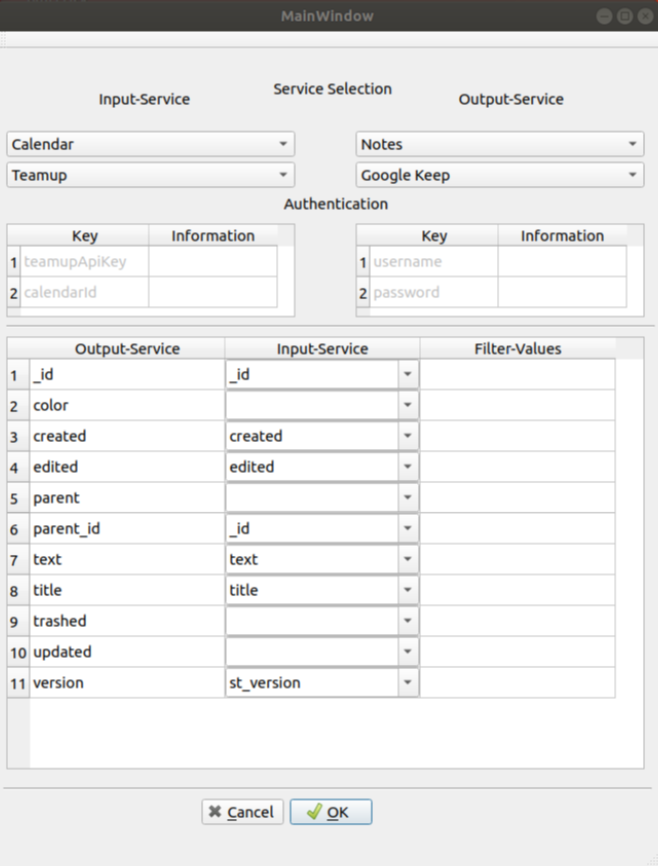
\includegraphics[width=0.6\textwidth]{pics/gui.png}	
	\caption{Graphische Benutzeroberfläche des Systems}
	\label{fig:gui}
\end{figure}
Um den Benutzern den Einstieg in die Anwendung zu erleichtern, wurde eine einfache graphische Benutzeroberfläche mithilfe des QT-Creators erzeugt. Der QT-Creator bietet die Möglichkeit die View-Perspektive der Oberfläche per Drag\&Drop mit den gewünschten Elementen zu befüllen. Hierfür erzeugt der QT-Creator drei Dateien, eine für das Projekt, eine für den aktuellen Bearbeiter des Projekts und eine \glqq .ui\grqq{}-Datei, die den Aufbau der Oberfläche beinhaltet. Mithilfe des pyuic-Tools, dass mit dem PyQt-Paket installiert wird, lässt sich aus der .ui-Datei durch den Befehl \glqq pyuic -o output.py input.uic\grqq{} ein Python-Skript erzeugen, welches die selbe Oberfläche innerhalb einer Klasse, standardmäßig MainWindow, definiert, dies kann jedoch im QT-Creator geändert werden. Ebenso könnte statt dem Python-Skript auch eine C- oder C++-Datei erzeugt werden. \\
Da diese Datei jedoch automatisch generiert ist und nur die View, siehe Abb.\ref{fig:gui}, also keinerlei Logik, enthält, muss diese noch eingepflegt werden. Um die Fortschritte durch ein erneutes Generieren der Oberfläche nicht zu zerstören, erzeugt man eine neue Klasse, die von dieser Oberfläche erbt und implementiert die Logik in der neuen Klasse. \\
Für diese Anwendung soll ein Benutzer die Möglichkeit haben, die Daten von einem beliebigen Service zu extrahieren und in einen neuen Service zu schreiben. Welche Services es gibt, wird mittels Introspection ermittelt, hierbei wird zur Laufzeit unter anderem analysiert, welche Vererbungshierarchien existieren\cite{Chun.2001}. In diesem Projekt entspricht dies, der Findung aller Kindklassen für die Klasse baseApiInterface, nachdem alle zum Projekt gehörigen Python-Skripte importiert wurden. Die möglichen Kategorien und Services ergeben sich über die id\_tags, die in den jeweiligen Service-Klassen definiert werden. \\
Die Login-Informationen, die für einen Service benötigt werden, müssen im Attribut authInfo des Services definiert werden, die möglichen Attribute die in einen Service geschrieben werden können, werden über ein zugehöriges Daten-Objekt definiert und über die Verbindung in der Service-Klasse ausgelesen. Hierbei können in der GUI derzeit nur triviale und keine komplexen Attribute dargestellt werden. Die zugehörigen Attribute des Input-Services werden anhand der Namensähnlichkeit vorbelegt, um diese zu übertragen, hierbei ergeben sich jedoch mehrere mögliche Szenarien. Das erste ist, dass aufgrund der internen, geänderten Namensstruktur keine Werte übereinstimmen, somit müssen alle Mappings der Attribute manuell durchgeführt werden. In der zweiten Variante, wird verglichen, welche Namen der Attribute des Output- oder des Input-Service mit einer genauen Übereinstimmung im jeweils anderen vorkommen, hier erhält man die gemeinsamen Attribute, insofern diese identisch benannt sind. Im dritten Szenario werden beide Richtungen geprüft, ohne genaue Übereinstimmung. Hiermit erhält man eine maximal mögliche Überschneidung, wobei manche Attribute möglicherweise fehlerhaft belegt werden, da die Übereinstimmung zu gering ist. So kann beim Vorhandensein von zehn ID-Feldern jedes mit der gleichen ID vorbelegt sein. Egal welche Variante genutzt wird, ist eine manuelle Überarbeitung notwendig. Durch die Vielzahl an existierenden Attributen, fiel die Wahl jedoch auf die dritte Variante. Statt dem Mapping auf ein Attribut kann auch eine Konstante in das Feld eingetragen werden, zudem ist ein String-Filter setzbar, um die Daten-Objekte anhand gültiger Werte einzuschränken, dass nur diese in einen Service geschrieben werden.

